\documentclass{beamer}
\usecolortheme{dove}
\setbeamertemplate{navigation symbols}{}
\usepackage{amsmath,amssymb,amsfonts,amsthm, multicol, subfigure, color}
\usepackage{bm}
\usepackage{graphicx}
\usepackage{tabularx}
\usepackage{booktabs}
\usepackage{hyperref}
\usepackage{pdfpages}
\usepackage{xcolor}
\definecolor{seagreen}{RGB}{46, 139, 87}
\definecolor{ucla}{RGB}{39, 116, 174}
\definecolor{darkestblue}{RGB}{0, 59, 92}
\definecolor{gold}{RGB}{255, 209, 0}
\def\independenT#1#2{\mathrel{\rlap{$#1#2$}\mkern2mu{#1#2}}}
\newcommand\indep{\protect\mathpalette{\protect\independenT}{\perp}}
\def\log{\text{log}}
\newcommand\logit{\text{logit}}
\newcommand\iid{\stackrel{\text{iid}}{\sim}}
\newcommand\E{\text{E}}
\newcommand\V{\text{V}}
\renewcommand\P{\text{P}}
\newcommand{\Cov}{\text{Cov}}
\newcommand{\Cor}{\text{Cor}}
\newcommand\doop{\text{do}}


\usepackage{stackrel}
\usepackage{tikz}
\usetikzlibrary{arrows,shapes.arrows,positioning,shapes,patterns,calc}
\newcommand\slideref[1]{\vskip .1cm \tiny \textcolor{gray}{{#1}}}
\newcommand\red[1]{\color{red}#1}
\newcommand\blue[1]{\color{blue}#1}
\newcommand\gray[1]{\color{gray}#1}
\newcommand\seagreen[1]{\color{seagreen}#1}
\newcommand\purple[1]{\color{purple}#1}
\newcommand\orange[1]{\color{orange}#1}
\newcommand\black[1]{\color{black}#1}
\newcommand\white[1]{\color{white}#1}
\newcommand\teal[1]{\color{teal}#1}
\newcommand\magenta[1]{\color{magenta}#1}
\newcommand\Fuchsia[1]{\color{Fuchsia}#1}
\newcommand\BlueGreen[1]{\color{BlueGreen}#1}
\newcommand\bblue[1]{\textcolor{blue}{\textbf{#1}}}
\newcommand\bred[1]{\textcolor{red}{\textbf{#1}}}
\newcommand\bgray[1]{\textcolor{gray}{\textbf{#1}}}
\newcommand\bgreen[1]{\textcolor{seagreen}{\textbf{#1}}}
\newcommand\bref[2]{\href{#1}{\color{blue}{#2}}}
\colorlet{lightgray}{gray!40}
\pgfdeclarelayer{bg}    % declare background layer for tikz
\pgfsetlayers{bg,main} % order layers for tikz
\newcommand\mycite[1]{\begin{scriptsize}\textcolor{darkgray}{(#1)}\end{scriptsize}}
\newcommand{\tcframe}{\frame{
%\small{
\only<1|handout:0>{\tableofcontents}
\only<2|handout:1>{\tableofcontents[currentsection]}}
%}
}

\setbeamertemplate{footline}[frame number]


\usepackage[round]{natbib}
\bibliographystyle{humannat-mod}
\setbeamertemplate{enumerate items}[default]
\usepackage{mathtools}

\newcommand{\goalsframe}{\begin{frame}{Learning goals for today}
At the end of class, you will be able to:
\begin{enumerate}
\item Define a conditionally randomized experiment
\item Define conditional exchangeability
\item Define conditional average treatment effects and recognize their use in policy
\end{enumerate} \vskip .2in
\end{frame}}

\title{Conditional Exchangeability}
\author{Sociol 114}
\date{4 Feb 2025}

\begin{document}

\maketitle

\goalsframe

\section{Review of Exchangeability}

\begin{frame}
\huge
Review of exchangeability
\end{frame}

\begin{frame}{Exchangeable sampling from a population}
\begin{tikzpicture}[x = \textwidth, y = .9\textheight]
% POPULATION
\node[anchor = north, font = \bf, color = ucla, align = center] at (.15,1) {Population\\Outcomes};
\foreach \i in {.3,.4,.5,.6,.7,.8} {
	\draw[fill = ucla, draw = white] (.08,\i - .05) rectangle (.22,\i + .05) {};
}
\node[font = {\bf}, white] at (.15,.8) {$Y_\text{Maria}$};
\node[font = {\bf}, white] at (.15,.7) {$Y_\text{William}$};
\node[font = {\bf}, white] at (.15,.6) {$Y_\text{Rich}$};
\node[font = {\bf}, white] at (.15,.5) {$Y_\text{Sarah}$};
\node[font = {\bf}, white] at (.15,.4) {$Y_\text{Alondra}$};
\node[font = {\bf}, white] at (.15,.3) {$Y_\text{Jes\'us}$};
% RANDOMIZATION
\node[anchor = north, font = \bf, color = ucla, align = center] at (.4,1) {Randomized\\Sampling};
%\foreach \i in {.3,.4,.5,.6,.7,.8} {
%	\draw[fill = ucla, draw = white] (.4,\i) rectangle (6,\i + .1) {};
%}
\node[font = {\bf}, anchor = east, ucla] at (.5,.8) {$S_\text{Maria} = 1$};
\node[font = {\bf}, anchor = east, ucla] at (.5,.7) {$S_\text{William} = 0$};
\node[font = {\bf}, anchor = east, ucla] at (.5,.6) {$S_\text{Rich} = 0$};
\node[font = {\bf}, anchor = east, ucla] at (.5,.5) {$S_\text{Sarah} = 1$};
\node[font = {\bf}, anchor = east, ucla] at (.5,.4) {$S_\text{Alondra} = 0$};
\node[font = {\bf}, anchor = east, ucla] at (.5,.3) {$S_\text{Jes\'us} = 1$};
% SAMPLE
\node[anchor = north, font = \bf, color = ucla, align = center] at (.62,1) {Sampled\\Outcomes};
\foreach \i in {.3,.5,.8} {
	\draw[fill = ucla, draw = white] (.55,\i - .05) rectangle (.69,\i + .05) {};
}
\node[font = {\bf}, white] at (.62,.8) {$Y_\text{Maria}$};
%\node[font = {\bf}, white] at (.75,.75) {$Y_\text{William}$};
%\node[font = {\bf}, white] at (.75,.65) {$Y_\text{Rich}$};
\node[font = {\bf}, white] at (.62,.5) {$Y_\text{Sarah}$};
%\node[font = {\bf}, white] at (.75,.45) {$Y_\text{Alondra}$};
\node[font = {\bf}, white] at (.62,.3) {$Y_\text{Jes\'us}$};
%\draw[fill = darkgray] (.75,0) rectangle (2,1);
\node[anchor = north west, align = left] at (.75,1) {\textbf{Estimator:}\\Estimate the\\population mean\\by the sample mean};
\node[anchor = north west, align = left] at (.75,.65) {\textbf{Key assumption}:\\Sampled and\\unsampled units\\are \textbf{exchangeable}\\due to random\\sampling};
\node[anchor = north west, align = left] at (.75,.27) {$Y\indep S$};
\end{tikzpicture}
\end{frame}

\begin{frame}{Exchangeable treatment assignment} %Y0 AND Y1

\begin{tikzpicture}[x = \textwidth, y = .9\textheight]
% POPULATION
\node[anchor = north, font = \bf, color = ucla, align = center] at (.23,1.05) {Population\\Potential\\Outcomes};
\foreach \i in {.3,.4,.5,.6,.7,.8} {
	\draw[fill = ucla, draw = white] (.08,\i - .05) rectangle (.22,\i + .05) {};
	\draw[fill = gold, draw = white] (.24,\i - .05) rectangle (.38,\i + .05) {};
}
\node[font = {\bf}, white] at (.15,.8) {$Y^1_\text{Maria}$};
\node[font = {\bf}, white] at (.15,.7) {$Y^1_\text{William}$};
\node[font = {\bf}, white] at (.15,.6) {$Y^1_\text{Rich}$};
\node[font = {\bf}, white] at (.15,.5) {$Y^1_\text{Sarah}$};
\node[font = {\bf}, white] at (.15,.4) {$Y^1_\text{Alondra}$};
\node[font = {\bf}, white] at (.15,.3) {$Y^1_\text{Jes\'us}$};
\node[font = {\bf}, darkestblue] at (.31,.8) {$Y^0_\text{Maria}$};
\node[font = {\bf}, darkestblue] at (.31,.7) {$Y^0_\text{William}$};
\node[font = {\bf}, darkestblue] at (.31,.6) {$Y^0_\text{Rich}$};
\node[font = {\bf}, darkestblue] at (.31,.5) {$Y^0_\text{Sarah}$};
\node[font = {\bf}, darkestblue] at (.31,.4) {$Y^0_\text{Alondra}$};
\node[font = {\bf}, darkestblue] at (.31,.3) {$Y^0_\text{Jes\'us}$};
% RANDOMIZATION
\node[anchor = north, font = \bf, color = ucla, align = center] at (.51,1) {Randomized\\Treatment};
%\foreach \i in {.3,.4,.5,.6,.7,.8} {
%	\draw[fill = ucla, draw = white] (.4,\i) rectangle (6,\i + .1) {};
%}
\node[font = {\bf}, anchor = east, ucla] at (.61,.8) {$A_\text{Maria} = 1$};
\node[font = {\bf}, anchor = east, ucla] at (.61,.7) {$A_\text{William} = 0$};
\node[font = {\bf}, anchor = east, ucla] at (.61,.6) {$A_\text{Rich} = 0$};
\node[font = {\bf}, anchor = east, ucla] at (.61,.5) {$A_\text{Sarah} = 1$};
\node[font = {\bf}, anchor = east, ucla] at (.61,.4) {$A_\text{Alondra} = 0$};
\node[font = {\bf}, anchor = east, ucla] at (.61,.3) {$A_\text{Jes\'us} = 1$};
% SAMPLE
\node[anchor = north, font = \bf, color = ucla, align = center] at (.83,1) {Observed\\Outcomes};
\foreach \i in {.3,.5,.8} {
	\draw[fill = ucla, draw = white] (.68,\i - .05) rectangle (.82,\i + .05) {};
}
\foreach \i in {.4,.6,.7} {
	\draw[fill = gold, draw = white] (.84,\i - .05) rectangle (.98,\i + .05) {};
}
\node[font = {\bf}, white] at (.75,.8) {$Y^1_\text{Maria}$};
\node[font = {\bf}, darkestblue] at (.91,.7) {$Y^0_\text{William}$};
\node[font = {\bf}, darkestblue] at (.91,.6) {$Y^0_\text{Rich}$};
\node[font = {\bf}, white] at (.75,.5) {$Y^1_\text{Sarah}$};
\node[font = {\bf}, darkestblue] at (.91,.4) {$Y^0_\text{Alondra}$};
\node[font = {\bf}, white] at (.75,.3) {$Y^1_\text{Jes\'us}$};
%\node[anchor = north west, align = left] at (.75,1) {\textbf{Estimator:}\\Estimate the\\population mean\\$\E(Y^0)$ by the\\untreated sample mean};
%\node[anchor = north west, align = left] at (.75,.65) {\textbf{Key assumption}:\\Treated and\\untreated units\\are \textbf{exchangeable}\\due to random\\treatment assignment};
%\node[anchor = north west, align = left] at (.75,.27) {$Y^0\indep A$};
\end{tikzpicture}
\end{frame}

\section{Conditional Randomization}

\begin{frame}
\huge A \textbf{conditionally} randomized experiment
\end{frame}

\begin{frame}
\onslide<2->{\Large Does exchangeability hold? How would you analyze?\vskip .1in}
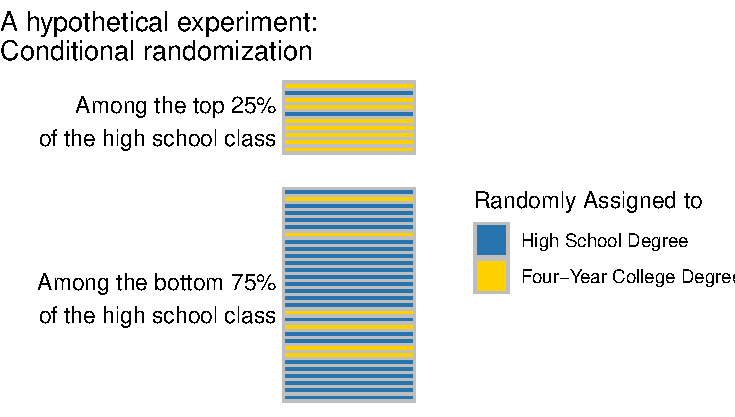
\includegraphics[width = \textwidth]{figures/conditional_randomization} \\
Outcome: Employed at age 40

\end{frame}

\begin{frame}{Conditional randomization: Exchangeability does not hold}

\begin{tikzpicture}[x = \textwidth, y =.8\textheight]
\node at (0,0) {};
\node at (1,1) {};
\node[anchor = south] at (.5,0) {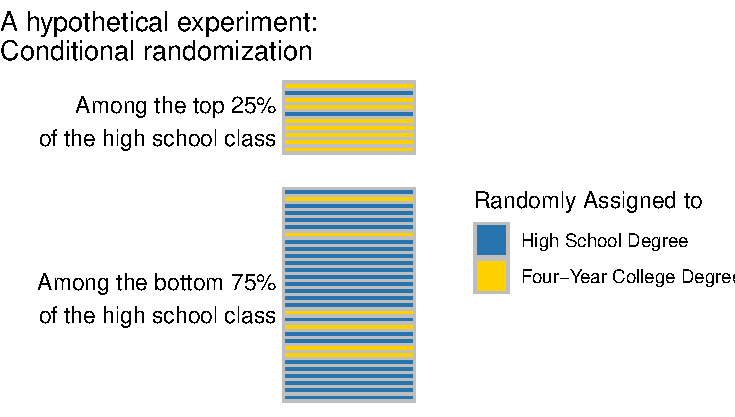
\includegraphics[width = .5\textwidth]{figures/conditional_randomization}};
\node<2->[anchor = north west, align = left, text width = \textwidth] at (0,1) {Treated units are more likely to have done well in high school};
\node<3->[anchor = north west, align = left, text width = \textwidth] at (0,.9) {Those who do well in high school are more likely to be employed at age 40 even without college};
\node<4->[anchor = north, font = \Large] at (.5,.75) {$\{Y^1,Y^0\}\not\indep A$};
\end{tikzpicture}

\end{frame}

\begin{frame}{Conditional randomization: Analyze within subgroups}

\begin{tikzpicture}[x = \textwidth, y =.8\textheight]
\node at (0,0) {};
\node at (1,1) {};
\node[anchor = south] at (.5,0) {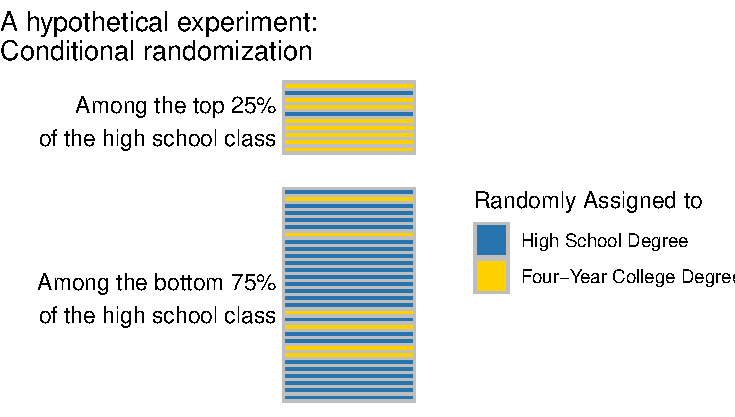
\includegraphics[width = .5\textwidth]{figures/conditional_randomization}};
\node<2->[anchor = north west, align = left, text width = \textwidth] at (0,1) {Among top 25\%, simple random experiment.\\Among bottom 75\%, simple random experiment.};
\node<3->[anchor = north west, align = left, text width = \textwidth] at (0,.85) {Conditional exchangeability:};
\node<3->[anchor = north, font = \Large] at (.5,.75) {$\underbrace{\{Y^1,Y^0\}}_{\substack{\text{Potential}\\\text{Outcomes}}} \underbrace{\indep}_{\substack{\text{Are}\\\text{Independent of}}} \underbrace{A}_\text{Treatment} \underbrace{\mid}_{\substack{\text{Within}\\\text{Subgroups}}} \underbrace{X}_\text{of X}$};
\end{tikzpicture}

\end{frame}

\begin{frame}{Conditional average treatment effects}

We get two estimates. Average effect of college on employment
\begin{itemize}
\item among those in the top 25\% of their high school class
\item among those in the bottom 75\% of their high school class
\end{itemize} \vskip .2in
These are \textbf{conditional average treatment effects}
$$
\underbrace{\tau(x)}_{\substack{\text{Conditional}\\\text{Average}\\\text{Treatment}\\\text{Effect}\\\text{(CATE)}}} = \underbrace{\text{E}}_{\substack{\text{Expected}\\\text{value of}}}\bigg(\underbrace{Y^1-Y^0}_\text{treatment effect} \quad \underbrace{\mid}_{\substack{\text{within the}\\\text{subgroup}\\\text{for whom}}} \quad \underbrace{\vec{X} = \vec{x}}_{\substack{\text{the predictors }\vec{X}\\\text{take the value }\vec{x}}}\bigg)
$$

\end{frame}

\begin{frame}{Effect heterogeneity: CATEs differ across subgroups}

Why might the effect of college on future employment
\begin{itemize}
\item be larger for those from the top 25\% of the high school class?
\item be larger for those from the bottom 75\% of the high school class?
\end{itemize}

\end{frame}

\begin{frame}{Effect heterogeneity and policy}

Suppose we study (college $\rightarrow$ employment) in two subgroups
\begin{itemize}
\item Advantaged subgroup
\begin{itemize}
\item Both parents finished college
\item Top quartile of family income at age 14
\item Took college prep courses
\end{itemize}
\item Disadvantaged subgroup
\begin{itemize}
\item Neither parent finished college
\item Bottom quartile of family income at age 14
\item Took college prep courses
\end{itemize}
\end{itemize} \vskip .1in
Discuss:
\begin{enumerate}
\item Whose CATE would be larger?
\item How might the difference inform policy?
\end{enumerate}

\end{frame}



\goalsframe

\end{document}

